Table~\ref{tab:spec} and Fig.~\ref{fig:specfig} compare speculative decoding with ordinary KV-cached greedy decoding of the same fine-tuned target on three validation prompts (different patients), for two workloads: \emph{task} (the real screening prompt; the JSON answer has 14 tokens and stops at \texttt{<|im\_end|>}) and \emph{long} (EOS disabled, 64 new tokens). The draft is the base SmolLM2-135M-Instruct; $k\in\{1,2,4\}$; one warm-up and two timed runs per configuration.

\textbf{Correctness.} All 18 speculative runs produced exactly the same token sequence as greedy decoding of the target, for every $k$; unit tests add three more $k$ values and a self-drafting test (target used as its own draft) in which, as expected, every drafted token is accepted. The invariant-based cache handling---cropping the target cache to the committed prefix after each verification and letting the draft cache lag by at most one token---is what makes this exact. As an external reference we also ran Hugging Face assisted generation with the same models; it stopped after 5 tokens whereas our greedy and speculative decoders produced the full 14-token answer, so this cross-check was inconclusive (most likely a difference in how the merged LoRA weights or the stop token were passed to the library) and we rely on equality with our own verified greedy path instead.

\begin{table}[t]\centering\caption{Speculative vs.\ greedy decoding (target: fine-tuned SmolLM2-360M; draft: SmolLM2-135M). Acc.\ = accepted/drafted tokens; tok/pass = committed tokens per target forward; speed-up = greedy latency / speculative latency (mean over prompts).}\label{tab:spec}
\setlength{\tabcolsep}{3pt}
\begin{tabular}{lcccccc}\toprule
Draft & $k$ & Same & Acc. & tok/pass & tok/s & Speed-up\\\midrule
\multicolumn{7}{l}{\textit{task workload} (3 prompts, mean new tokens 14; greedy 3.1 tok/s)} \\
base\_135m & 1 & yes & 0.625 & 1.56 & 2.5 & 0.76 \\
base\_135m & 2 & yes & 0.667 & 2.00 & 3.5 & 1.14 \\
base\_135m & 4 & yes & 0.364 & 2.00 & 2.4 & 0.79 \\
\multicolumn{7}{l}{\textit{long workload} (3 prompts, mean new tokens 64; greedy 3.8 tok/s)} \\
base\_135m & 1 & yes & 0.863 & 1.83 & 4.6 & 1.24 \\
base\_135m & 2 & yes & 0.825 & 2.57 & 4.7 & 1.25 \\
base\_135m & 4 & yes & 0.690 & 3.53 & 5.1 & 1.38 \\
\bottomrule\end{tabular}\end{table}

\begin{figure}[t]\centering
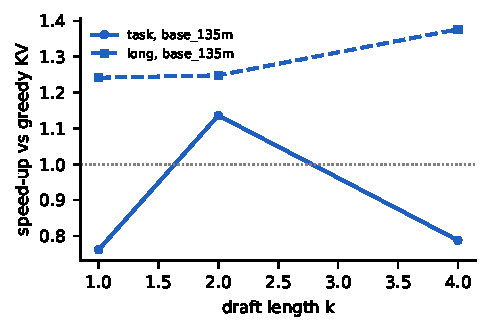
\includegraphics[width=\columnwidth]{figures/spec_speedup.pdf}
\caption{Mean speed-up of speculative over greedy decoding as a function of draft length $k$ for the short task answers and 64-token generation.}\label{fig:specfig}
\end{figure}

\textbf{Efficiency.} On long generation the draft agrees with the target on 86\% of drafted tokens at $k{=}1$ and 69\% at $k{=}4$, so each target pass commits 1.8--3.5 tokens and speculative decoding is 1.24--1.38$\times$ faster on average (up to 1.63$\times$ on one prompt). On the short task answers it is mostly \emph{slower} (0.76$\times$ at $k{=}1$, 0.79$\times$ at $k{=}4$; only $k{=}2$ gains, 1.14$\times$). Three effects explain this. (i) The cost ratio is unfavourable: a decode step of either model is memory-bandwidth bound, so the 135M draft costs roughly its share of weight bytes, $pprox$37\% of a 360M target pass (0.54 vs.\ 1.45\,GB), whereas the expected speed-up of speculative decoding grows as the draft-to-target cost ratio shrinks~\cite{leviathan2023fast}. (ii) With only 14 output tokens, the fixed costs---prefilling the draft as well as the target, and the first token that must come from the target---are amortised over very few tokens. (iii) The base draft was not fine-tuned, so it disagrees with the fine-tuned target exactly on the informative label tokens (acceptance 36\% at $k{=}4$ on the task workload); a longer $k$ then wastes draft passes on rejected tokens. Memory overhead is the second model (0.54\,GB fp32) plus its cache (45\,KiB/token). A fine-tuned draft, smaller drafts (e.g.\ layer-skipping self-speculation) or batch serving on a GPU, where the target pass is compute-light relative to its fixed overhead, are the natural ways to turn the measured acceptance into speed.
